%\documentclass[tikz, border=10pt]{standalone}
%\usepackage{tikz}
%\usetikzlibrary{positioning}

%\begin{document}

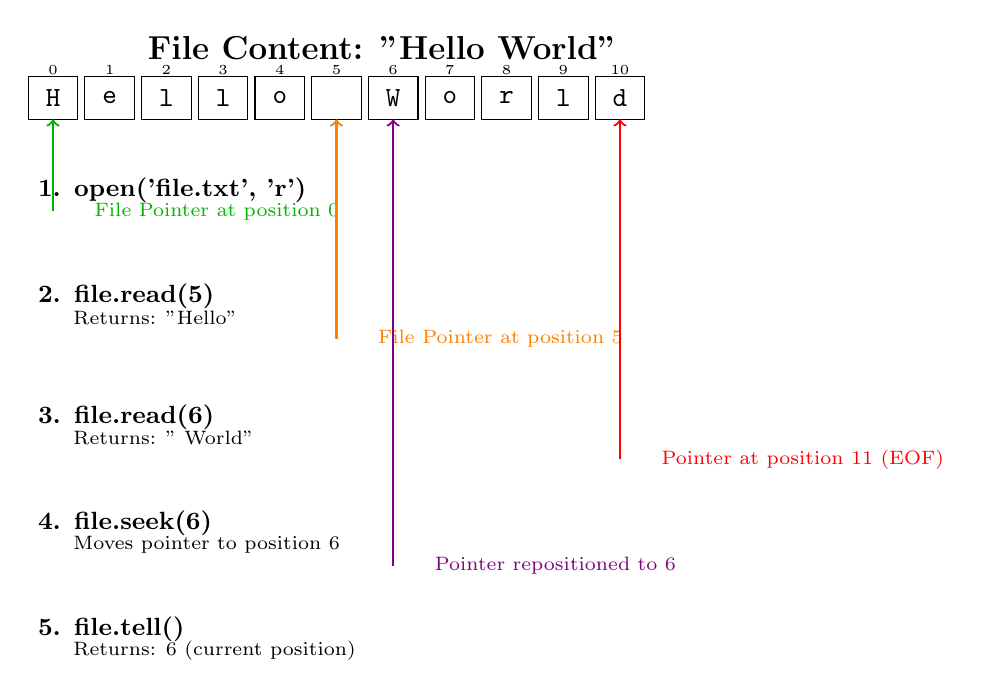
\begin{tikzpicture}[scale=0.9]
    
    % Title
    \node[font=\large\bfseries] at (5, 7) {File Content: "Hello World"};
    
    % Character boxes with positions
    \foreach \i/\char in {0/H, 1/e, 2/l, 3/l, 4/o, 5/{ }, 6/W, 7/o, 8/r, 9/l, 10/d} {
        \draw (\i*0.8, 6) rectangle ++(0.7, 0.6);
        \node at (\i*0.8+0.35, 6.3) {\texttt{\char}};
        \node[font=\tiny] at (\i*0.8+0.35, 6.7) {\i};
    }
    
    % State 1: Opening file
    \node[anchor=west, font=\small\bfseries] at (0, 5) {1. open('file.txt', 'r')};
    \draw[->, thick, green!70!black] (0.35, 4.7) -- (0.35, 6);
    \node[anchor=west, font=\scriptsize, green!70!black] at (0.8, 4.7) {File Pointer at position 0};
    
    % State 2: After reading 5 characters
    \node[anchor=west, font=\small\bfseries] at (0, 3.5) {2. file.read(5)};
    \node[anchor=west, font=\scriptsize] at (0.5, 3.2) {Returns: "Hello"};
    \draw[->, thick, orange] (4.35, 2.9) -- (4.35, 6);
    \node[anchor=west, font=\scriptsize, orange] at (4.8, 2.9) {File Pointer at position 5};
    
    % State 3: After reading more
    \node[anchor=west, font=\small\bfseries] at (0, 1.8) {3. file.read(6)};
    \node[anchor=west, font=\scriptsize] at (0.5, 1.5) {Returns: " World"};
    \draw[->, thick, red] (8.35, 1.2) -- (8.35, 6);
    \node[anchor=west, font=\scriptsize, red] at (8.8, 1.2) {Pointer at position 11 (EOF)};
    
    % State 4: seek() operation
    \node[anchor=west, font=\small\bfseries] at (0, 0.3) {4. file.seek(6)};
    \node[anchor=west, font=\scriptsize] at (0.5, 0) {Moves pointer to position 6};
    \draw[->, thick, violet] (5.15, -0.3) -- (5.15, 6);
    \node[anchor=west, font=\scriptsize, violet] at (5.6, -0.3) {Pointer repositioned to 6};
    
    % State 5: tell() operation
    \node[anchor=west, font=\small\bfseries] at (0, -1.2) {5. file.tell()};
    \node[anchor=west, font=\scriptsize] at (0.5, -1.5) {Returns: 6 (current position)};
    
\end{tikzpicture}

%\end{document}
